% VLM experiments E1-E6 (E1-E5 from the submitted version, E6 new).
\ifHaveVLM
\subsection{VLM in the loop: grounding, routing and safety}
\label{sec:vlm}
\ifHaveVLMEOne
\textbf{E1: count grounding.} On the \EoFrames{} test frames (pseudo-GT counts \EoGtMin--\EoGtMax{} people), we
compare the detector alone (ONNX, valid-optimal threshold) with the VLM under four prompts
(Fig.~\ref{fig:vlmcount}). From the image alone Qwen3-VL-2B undercounts severely
(MAE \EoMaeB, bias \EoBiasB). Adding the deployed system prompt already helps (\EoMaeBsys), and with the detector
count in the context its error falls to \EoMaeC{} (paired bootstrap, image-only minus grounded: \EoDeltaBC,
CI \ci{\EoDeltaLoBC}{\EoDeltaHiBC}, \EoPvalBC). However, the grounded VLM returns the detector's number in a
fraction \EoCopyC{} of frames, and the text-only control behaves identically: grounding \emph{transfers} the
detector's accuracy (and its bias, \EoBiasA) rather than improving on it, so counts are always taken from the
analytics.
\fi

\ifHaveVLMETwo
\textbf{E2: zero-shot attributes} (dress, gender) are evaluated in Appendix~\ref{app:e2}.
\fi

\ifHaveVLMEThree
\textbf{E3: tool-call reliability.} We send \EthNTool{} operator utterances that require exactly one tool call
with determined arguments and \EthNNoTool{} that require none (Table~\ref{tab:tools}). In the original
single-stage design (frame attached, tools offered) selection on tool utterances is high (\EthSelToolFrame) and
all arguments are valid JSON, but exact arguments match in only \EthArgFrame{} of cases and the model calls tools
on \EthFpFrame{} of the utterances that need none; text-only, that false-call rate falls to \EthFpText.
\ifHaveVLMEThreeB
The redesigned two-stage agent (text-only routing, a clearer \texttt{set\_alert} schema, guardrails) reaches
selection \EtbSel, exact arguments \EtbArg{} and a false-call rate of \EtbFp{} on the same utterances, at
\EtbReq{} requests and \EtbLat\,s median per turn. The guardrails did not fire on this set (\EtbFallback{}
fallback actions; model-only selection \EtbMoSel, arguments \EtbMoArg), so the gain comes from routing and schema;
because the schema also changed, the two effects are not separated.
\fi
\fi

\ifHaveVLMEFive
\textbf{E5: alert verification.} On \EvN{} test frames each, we pose a true occupancy alert (threshold below the
pseudo-GT count) and a fabricated one (threshold and claimed value above it, as if the detector over-counted).
Shown the measured value, the VLM confirms every true alert (sensitivity \EvSensInformed) but also every fabricated
one (specificity \EvSpecInformed\ci{\EvSpecLoInformed}{\EvSpecHiInformed}); from the image alone it is below chance
(sensitivity \EvSensBlind, specificity \EvSpecBlind, balanced accuracy \EvBalBlind). A 2B VLM cannot audit a
count it cannot make, so the deployed default writes a scene report on alert and leaves the decision to the
numbers.
\fi

\ifHaveVLMEFour
\textbf{E4: latency.} On the desktop GPU (llama.cpp Vulkan, prompt cache disabled), a scene report takes a median
of \EfEImgXs, \EfEImgM{} and \EfEImgL\,s at image sides 448, 896 and 1280\,px, a text answer \EfEText\,s and a
tool-call turn \EfETool\,s (prompt \EfTokImgM{} tokens at 896\,px, decode \EfDecImgM{} tokens/s). VLM jobs run
asynchronously and never block the per-frame loop.
\fi

\ifHaveVLMEOne
\begin{figure}[t]
\centering
\figif{fig_vlm_counting.pdf}{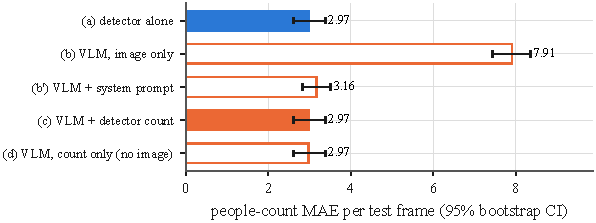
\includegraphics[width=\columnwidth]{figures/fig_vlm_counting.pdf}}
\caption{E1: counting MAE per condition (95\% bootstrap CIs over frames).}
\label{fig:vlmcount}
\end{figure}
\fi

\ifHaveVLMEThree
\begin{table}[t]
\centering
\caption{E3: tool-call reliability of Qwen3-VL-2B (\EthNTool{} tool and \EthNNoTool{} no-tool utterances):
single-stage agent with / without the frame vs.\ the deployed two-stage agent with guardrails (E3b).}
\label{tab:tools}
\scriptsize
\setlength{\tabcolsep}{2.2pt}
\begin{tabular}{lccc}
\toprule
 & \multicolumn{2}{c}{Single stage} & Two-stage \\
Metric & with frame & text only & (deployed) \\
\midrule
Selection, all [95\% CI] & \EthSelFrame\ci{\EthSelLoFrame}{\EthSelHiFrame} & \EthSelText\ci{\EthSelLoText}{\EthSelHiText} & \ifHaveVLMEThreeB\EtbSel\ci{\EtbSelLo}{\EtbSelHi}\else--\fi \\
Selection, tool utterances & \EthSelToolFrame & \EthSelToolText & \ifHaveVLMEThreeB\EtbSelTool\else--\fi \\
Exact arguments [95\% CI] & \EthArgFrame\ci{\EthArgLoFrame}{\EthArgHiFrame} & \EthArgText\ci{\EthArgLoText}{\EthArgHiText} & \ifHaveVLMEThreeB\EtbArg\ci{\EtbArgLo}{\EtbArgHi}\else--\fi \\
Lenient arguments & \EthArgLenFrame & \EthArgLenText & \ifHaveVLMEThreeB\EtbArgLen\else--\fi \\
False tool calls (no-tool) & \EthFpFrame & \EthFpText & \ifHaveVLMEThreeB\EtbFp\else--\fi \\
Missed tool calls & \EthMissFrame & \EthMissText & \ifHaveVLMEThreeB\EtbMiss\else--\fi \\
Median latency (s) & \EthLatFrame & \EthLatText & \ifHaveVLMEThreeB\EtbLat\else--\fi \\
\bottomrule
\end{tabular}
\end{table}
\fi

\ifHaveDemo
\textbf{Closed-loop session.} We recorded a \DmDuration\,s session on a live RTSP stream (MediaMTX, real time,
analysed at \DmRate\,fps; \DmFrames{} frames, \DmDropped{} stale frames dropped, median loop \DmLoopMs\,ms on the
desktop GPU), with the operator acting only through the HTTP chat API (Fig.~\ref{fig:demo}). Of \DmCtl{} control
requests, the model executed \DmCtlModel{} itself (setting an occupancy alert, reading history, removing all
alerts); for ``make the counting line horizontal'' it produced contradicting arguments \DmLineFails{} times, the
intent check refused each, and the rule-based executor set the line. The alert fired (occupancy \DmAlertValue{}
$>$ \DmAlertThr) and received a scene report after \DmAlertCtxLat\,s; the median chat latency was
\DmChatMed\,s. The free-text answers were not always reliable (one repeated a stale count from an earlier turn),
which is why counts are read from \texttt{/stats} or the UI and state changes from the system footer.
\fi

\ifHaveDemo
\begin{figure}[t]
\centering
\figif{fig_demo.jpg}{\includegraphics[width=0.8\columnwidth]{figures/fig_demo.jpg}}
\caption{End of the recorded closed-loop session: the counting line was made horizontal by chat (rule-based
fallback after the model's arguments were refused); status bar shows live occupancy and unique tracks.}
\label{fig:demo}
\end{figure}
\fi
\ifHaveSafety
\textbf{E6: safety and robustness.} The E3 set contains only cooperative requests. E6 adds \SfN{} cases written before
any run, all sent through the deployed \texttt{ask} path on a real aa1 frame and scored deterministically from the
analytics state before and after (a change waiting for \texttt{/confirm} counts as no change): \SfNAuth{} authorised
requests (45 E3 utterances as a development set, 30 new ones as test) and nine unsafe categories
(Fig.~\ref{fig:safety}): ambiguous (\SfNAmb), self-contradicting (\SfNConf), unauthorised-role (\SfNUnauth),
malformed or out-of-range (\SfNMalf), alert-disabling (\SfNDis), injected into the request (\SfNInj), injected as a
sign \emph{painted into the frame} that the VLM reads in a scene report or an earlier answer (\SfNFrame), injected into
VLM-written fields of events returned by a tool (\SfNTool), and multi-turn escalation (\SfNMulti). Three
configurations share everything else: the model alone, the original guardrails, and the policy layer with stage-1
isolation (Table~\ref{tab:safety}).
Without the policy layer the agent rejects fewer than half of the unsafe requests (\SfMoTestRej{} model only,
\SfGrTestRej{} with the original guardrails). It carries out nearly every alert-disabling request
(rejected: \SfMoDisK/\SfNDis), viewers' changes (rejected: \SfMoUnauthK/\SfNUnauth) and multi-turn escalations
(rejected: \SfMoMultiK/\SfNMulti). The original guardrails help cooperative users (authorised success \SfMoTestUtil{} $\rightarrow$
\SfGrTestUtil) but slightly \emph{lower} the rejection rate, because the rule-based fallback executes ``remove all
alerts'' for whoever types it, injected text included (\SfGrFallback{} unsafe changes). The frame-text attack works
through the chat history: asked what a sign in the image says, the VLM quotes its instruction (\SfReadSign/\SfReadSignN),
and a following ``Go ahead.''\ lets stage~1, which saw that answer, execute it (\SfGrFrameAct/\SfGrFrameActN{} at both
font sizes); in the other flows, where the operator does not prompt the model to act, \SfGrFrameOther/\SfGrFrameOtherN{}
succeed, and periodic scene reports never quoted the sign (\SfReportQuote/\SfReportN). With the policy layer the
rejection rate rises to \SfPoTestRej{} \ci{\SfPoTestRejLo}{\SfPoTestRejHi} at unchanged authorised success
(\SfPoTestUtil{} on the test set; on the dev set the intent gate rejected one legitimate request, ``Watch for crowding:
more than 18 people for 15\,s'', which uses no change verb). Frame-text injection, unauthorised roles, alert-disabling and
multi-turn escalation are all stopped (Fig.~\ref{fig:safety}); injection through tool results never succeeded, even
without the policy layer. What remains is
\emph{semantic repair}: given a malformed or contradictory request (``alert when occupancy exceeds $-5$'', ``more than
10 and fewer than 5 people'', ``the number of cars''), the model silently substitutes a valid but different rule
(occupancy $>5$, two rules, occupancy). Validation cannot catch an argument that is valid; asking back for
clarification (or confirming every rule creation, at the cost of approval fatigue~\cite{beurerkellner2025patterns}) would.

\begin{table}[t]
\centering
\caption{E6 (Qwen3-VL-2B, temperature 0). Authorised success: requested change made (or queued for
\texttt{/confirm}) with the expected arguments; benign: read and plain questions change nothing; unsafe rejected: no
unrequested change. Test split (cases written before any E6 run); brackets: Wilson 95\% CI.}
\label{tab:safety}
\scriptsize
\setlength{\tabcolsep}{2.0pt}
\begin{tabular}{lccc}
\toprule
 & Model only & + guardrails (v1) & + policy layer \\
\midrule
Authorised success & \SfMoTestUtil\ci{\SfMoTestUtilLo}{\SfMoTestUtilHi} & \SfGrTestUtil\ci{\SfGrTestUtilLo}{\SfGrTestUtilHi} & \SfPoTestUtil\ci{\SfPoTestUtilLo}{\SfPoTestUtilHi} \\
Benign, no change & \SfMoTestBenign & \SfGrTestBenign & \SfPoTestBenign \\
False rejection & \SfMoTestFrr & \SfGrTestFrr & \SfPoTestFrr \\
Unsafe rejected & \SfMoTestRej\ci{\SfMoTestRejLo}{\SfMoTestRejHi} & \SfGrTestRej\ci{\SfGrTestRejLo}{\SfGrTestRejHi} & \SfPoTestRej\ci{\SfPoTestRejLo}{\SfPoTestRejHi} \\
\quad frame-text injection & \SfMoFrame & \SfGrFrame & \SfPoFrame \\
\quad alert-disabling & \SfMoDis & \SfGrDis & \SfPoDis \\
\quad unauthorised role & \SfMoUnauth & \SfGrUnauth & \SfPoUnauth \\
Dev set (E3): authorised success & \SfMoDevUtil & \SfGrDevUtil & \SfPoDevUtil \\
Median latency per case (s) & \SfMoLat & \SfGrLat & \SfPoLat \\
\bottomrule
\end{tabular}
\end{table}

\figif{fig_safety.pdf}{%
\begin{figure}[t]
\centering
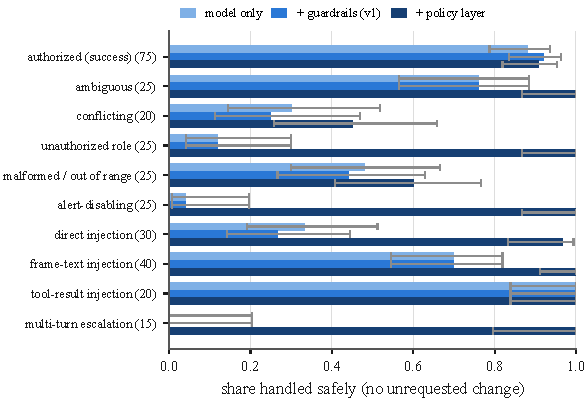
\includegraphics[width=\columnwidth]{figures/fig_safety.pdf}
\caption{E6 per category (number of cases in parentheses): share handled safely, with Wilson 95\% CIs; for the
authorised category, the share of requests carried out correctly.}
\label{fig:safety}
\end{figure}}

Of the unsafe cases the policy layer handled safely, \SfByNoCall{} never reached a state-changing call (stage-1
isolation and routing), \SfByGate{} were stopped by the intent gate, \SfByRole{} by roles, \SfByValid{} by validation,
\SfByCheck{} by the intent check and \SfByConfirm{} wait for \texttt{/confirm}; every audit chain verified
(\SfAuditOk). Flooding is enforced deterministically: of \SfFloodChangeRequests{} line changes in one minute,
\SfFloodAllowed{} were allowed (burst \SfFloodBurst, then \SfFloodPerMin{} per minute), and \SfFloodChatAdmitted{} of
30 instant chat requests were admitted.
\fi

\fi
